\documentclass[tikz,crop]{standalone}
\usetikzlibrary{angles,quotes,positioning,arrows,shapes,patterns,decorations,calc,decorations.pathreplacing}
\usepackage{mathptmx}
\usepackage[T1]{fontenc}
\usepackage{pgfplots}
\pgfplotsset{compat=1.18}
\usepackage{mathrsfs}
\tikzset{
  treenode/.style = {shape=rectangle, rounded corners,
                     draw, align=center,
                     top color=white, bottom color=blue!20},
  root/.style     = {treenode, font=\Large, bottom color=red!30,text width = 12em},
  env/.style      = {treenode, font=\normalsize,text width = 12em},
  dummy/.style    = {circle,draw},
}
\begin{document}
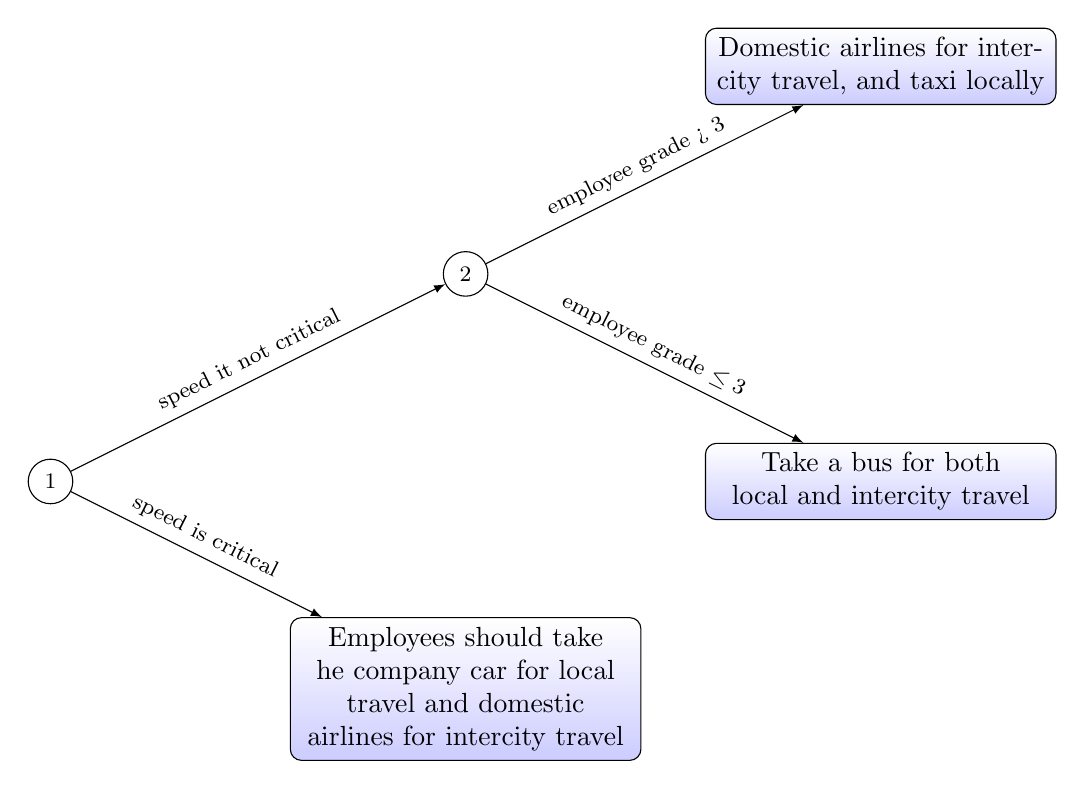
\begin{tikzpicture}[
        grow                    = right,
        sibling distance        = 15em,
        level distance          = 15em,
        edge from parent/.style = {draw, -latex},
        every node/.style       = {font=\footnotesize},
        sloped
    ]
    \node [dummy] {1}
    child{ node [env] {Employees should take he company car for local travel and domestic airlines for intercity travel}
            edge from parent node [above] {speed is critical}}
    child{node [dummy]{2}
            child{node [env]{Take a bus for both local and intercity travel}
                    edge from parent node [above] {employee grade \(\le 3\)}}
            child{
                    node [env]{Domestic airlines for intercity travel, and taxi locally}
                    edge from parent node [above] {employee grade > 3}
                }
            edge from parent node [above] {speed it not critical}};
\end{tikzpicture}
\end{document}